\chapter{Methodology}  \label{sec:method}

The \ac{dea} is a novel attack method that extends the capabilities of \ac{gma}s by moving beyond the intersection of datasets to re-identify individuals who were previously unmapped.
This chapter outlines the methodology behind the \ac{dea}, including modifications to the \ac{gma}, the design and implementation of the \ac{dea} itself, and the use of \ac{ann}s to enable probabilistic reconstruction of \ac{pii} from encoded data.

The \ac{dea} builds upon the \ac{gma} by using its re-identification results as a foundation for further inference.
While the \ac{gma} re-identifies only those records that exist in both the attacker’s dataset and the encoded target dataset, it often leaves a substantial portion of records unmapped.
The goal of the \ac{dea} is to extend this re-identification process by applying a machine learning–based approach to infer the missing \ac{pii} of the remaining records using a trained \ac{ann}.

To achieve this, the \ac{dea} follows a structured pipeline comprising six key steps, as illustrated in Figure~\ref{fig:deaoverview}.
The first step involves executing the \ac{gma} and extracting its results in a predefined format to serve as training data.
This dataset includes the re-identified individuals, their corresponding encoded representations, and the plaintext information that was successfully linked.
In addition, the \ac{gma} results contain the non-re-identified individuals, who are represented solely by their encoded \ac{pii} and associated plaintext values.

\begin{figure}[H]
    \centering
    \includegraphics[width=0.7\textwidth, page=15]{img/visualization.pdf}
    \caption{Overview of the \ac{dea} attack pipeline.}
    \label{fig:deaoverview}
\end{figure}

Once the data is extracted, it undergoes a transformation process to prepare it for \ac{ann} training.
This data preparation step involves constructing specialized datasets that convert the encoded representations and their corresponding labels—plaintext $n$-grams—into tensor-based formats suitable for processing by deep learning models.
The resulting datasets are subsequently split into training, validation, and test subsets, and corresponding data loaders are created to facilitate efficient mini-batch processing during model training.

With the data pipeline in place, a hyperparameter optimization is conducted to identify the best-performing model configuration.
This process systematically evaluates various combinations of hyperparameters, including the number of hidden layers, layer widths, activation functions, optimizers, and learning rate schedulers.
The optimal hyperparameters are then used to define the \ac{ann} architecture, which is trained to learn the mapping between encoded representations and their corresponding plaintext $n$-grams.

The architecture of the \ac{ann} is tailored to the specific characteristics of the encoding schemes used in the \ac{pprl} scheme.
The input layer size is determined by the dimensionality of the encoded representation, while the output layer size corresponds to the size of the predefined $n$-gram dictionary.

Once the best hyperparameter configuration is identified, the \ac{ann} is trained using the re-identified individuals as labeled data.
Training proceeds over multiple epochs, during which the model iteratively processes the training dataset, computes the loss, and updates its parameters via backpropagation.
Performance is continuously monitored on the validation set to track generalization and prevent overfitting.

Once the \ac{ann} is trained, it can be applied to the set of non-re-identified individuals, i.e., records that remained unmapped after the \ac{gma}.
This dataset serves as the test set during the experimentation phase to evaluate the performance of the attack.

The model outputs a probability distribution over all possible n-grams for each entry, indicating the likelihood of each n-gram being present in the corresponding plaintext data.
To refine these predictions, a thresholding mechanism is applied to filter out low-confidence outputs and retain only the most probable n-grams.
These predicted n-grams are then aggregated and reconstructed into potential \ac{pii}, constituting the final step of the \ac{dea} process.

This methodological approach represents a significant advancement in attacking \ac{pprl} systems.
By leveraging deep learning techniques, the \ac{dea} enables an attacker to infer sensitive personal information beyond the scope of traditional \ac{gma} approaches.
The following sections provide a detailed discussion of each component, including the design choices, implementation details, and challenges encountered during development.

\section{Problem Definition} \label{sec:problemdefinition}

The primary challenge that the \ac{dea} seeks to address is the limited scope of re-identifications achieved by the \ac{gma}.
While the \ac{gma} effectively links records by exploiting structural relationships within encoded datasets, its success is inherently restricted to individuals who are present in both the plaintext and the encoded datasets and can be matched based on graph similarity.
However, in real-world scenarios, there may exist additional re-identification potential beyond these direct matches.

One possible way to extend re-identifications is to rerun the \ac{gma} iteratively, incorporating additional publicly available data to gradually refine the matching process.
However, this approach is inherently dependent on the availability and quality of external data sources, which may not always be feasible.
Instead, the \ac{dea} introduces a novel strategy that aims to reconstruct deterministic relationships between encoded representations and their corresponding plaintext information.
This is based on the observation that all encoding schemes used in \ac{pprl} rely on hash functions or other deterministic mappings.

Hash functions, for example, produce fixed-length outputs from inputs of arbitrary length and, crucially, are deterministic — meaning the same input will always yield the same output.
The \ac{dea} leverages this property by training \ac{ann}s to learn statistical relationships between encoded values and the original n-grams of \ac{pii}.
The objective is to recover the most probable plaintext representation given an encoded input, effectively framing the attack as a probabilistic, frequency-based inference problem.
However, several challenges complicate this task.

The first major challenge is the lack of knowledge about the specific number and type of hash functions used during encoding.
As a result, the model must learn patterns in the data without any explicit understanding of the underlying hashing mechanisms.
Fortunately, this limitation is partially mitigated by the fact that the \ac{dea} does not rely on a one-to-one mapping between hash outputs and plaintext n-grams, but instead depends on statistical inference across large numbers of training samples.

A more fundamental challenge arises from the collision property of hash functions.
Because hash functions map an infinite input space to a finite output space, different inputs may produce identical hash values, making it inherently difficult to perfectly recover the original plaintext.
These collisions introduce uncertainty into the re-identification process, preventing the \ac{dea} from achieving perfect reconstruction accuracy.
Consequently, the predictions made by the \ac{dea} are probabilistic rather than deterministic — it can estimate the likelihood of a specific n-gram being present in the original \ac{pii}, but cannot guarantee absolute correctness.

The primary reason the \ac{gma} alone is unable to achieve such probabilistic reconstruction is that it relies solely on structural similarities within the dataset, without attempting to infer direct relationships between encoded values and their plaintext equivalents.
In contrast, the \ac{dea} enhances the capabilities of the \ac{gma} by enabling the reconstruction of individual plaintext components directly from encoded representations, thereby increasing the overall re-identification potential.
This novel approach significantly improves the effectiveness of the attack, allowing for the re-identification of individuals who were previously unmatchable using traditional graph-based techniques.


\section{Attacker Model}

The attacker in the \ac{dea} scenario is modeled as the linkage unit within a \ac{pprl} protocol.
This aligns with standard threat models in the literature, where the linkage unit is typically assumed to be semi-honest or honest-but-curious—faithfully executing the prescribed protocol while remaining interested in extracting sensitive information from the encoded data it processes \cite{schnell2009privacy, vatsalan2017privacy}.

Following Kerckhoffs’s principle, the attacker is assumed to possess full knowledge of the \ac{pprl} system design, including encoding algorithms (e.g., Bloom filter construction), parameter settings (e.g., filter length, n-gram size, number of hash functions), and record linkage procedures.
However, any dataset-specific secrets — such as cryptographic keys, random seeds, or salt values — are assumed to be unknown to the attacker.

In this setting, the attacker is presented with two encoded datasets — originating from, for example, two organizations engaging in privacy-preserving linkage — and aims to re-identify individuals across them.

The attacker is assumed to operate in an offline setting without time constraints, allowing the use of exhaustive search, large-scale training, and iterative optimization.
Given that linkage units are often embedded in national statistical agencies, health departments, or research consortia, it is realistic to assume access to powerful computational resources, including parallel processing and GPU acceleration.

The primary goal of the attacker is to maximize the overall re-identification rate, demonstrating that individuals not re-identified through traditional graph matching can still be decoded using more advanced techniques.
To evaluate the effectiveness of the \ac{dea}, its performance is compared to baseline strategies such as:

\begin{itemize}
    \item \textbf{Random guessing}, in which candidate plaintext values are assigned randomly to encodings.
    \item \textbf{Frequency-based decoding}, where common n-grams or token sets are mapped to frequent encoding patterns \cite{herzog2007data}.
\end{itemize}

These baselines represent naïve yet plausible strategies in the absence of supervised learning.
A successful \ac{dea} must significantly outperform these baselines to substantiate its threat to real-world \ac{pprl} deployments.


\section{Modular Design of the \ac{dea}} \label{sec:designandimplementation}

The \ac{dea} aims to reconstruct plaintext \ac{pii} from encoded records using machine learning techniques.
A central challenge in implementing the \ac{dea} lies in the diversity of encoding schemes used to protect sensitive data.
As each encoding method transforms plaintext into distinct numerical representations, the \ac{dea} must adapt both the dataset structure and the \ac{ann} architecture accordingly.

To address this, the \ac{dea} adopts a modular design: while the overall attack methodology remains consistent, specific implementations are tailored to each encoding scheme.
Although the input representation and network architecture vary depending on the encoding, the output format is kept uniform across all models.
The attack is framed as a multi-label classification task, where the \ac{ann} predicts the likelihood of individual n-grams appearing in the original \ac{pii}.
For each encoding scheme, a dedicated dataset structure transforms encoded records into a format suitable for \ac{ann} training.
Moreover, a custom \ac{ann} architecture is employed for each encoding scheme to ensure the model effectively learns the mapping from encoded data to plaintext n-grams.

\section{Step 1: \ac{gma}} \label{sec:deagma}

\subsection{Running the \ac{gma}} \label{sec:runninggma}

The \ac{gma} constitutes the first step in our \ac{dea} pipeline, establishing a critical foundation by identifying overlapping individuals between the encoded (target) dataset and the auxiliary (attacker) dataset.
It exploits structural similarities between records to perform graph-based matching and re-identification of individuals.

In this phase, we apply the adjusted \ac{gma} implementation by Schaefer et al.~\cite{schaefer2024}, which builds upon and extends the original approach introduced by Vidanage et al.~\cite{vidanage2020graph}.
This attack yields a partial mapping between records in the encoded dataset and plaintext identities from the auxiliary dataset.
The successfully re-identified individuals represent the known intersection between both datasets and serve as labeled training data for the inference component of the \ac{dea}.

The output of this step comprises two distinct sets of records:
(1) re-identified individuals, with known plaintext identities and their corresponding encoded representations, and
(2) non-re-identified individuals, whose encoded representations remain unmapped.
These unmapped encodings form the target set for the neural network-based reconstruction in the subsequent inference phase.

The effectiveness of the \ac{dea} is directly influenced by the quality of the \ac{gma} output.
A higher re-identification rate in the \ac{gma} provides a larger training set for the \ac{ann}, improving its ability to infer plaintext n-grams and reconstruct sensitive information for non-re-identified individuals.
Conversely, a low re-identification rate limits the availability of labeled data and diminishes the overall reconstruction capability of the \ac{dea}.

\subsection{Modifications to the \ac{gma}} \label{sec:modificationstogma}

To integrate the \ac{gma} as a preprocessing step for the \ac{dea}, modifications were made to the original implementation by Schaefer et al.~\cite{schaefer2024}.
While the core algorithm remains unchanged, adjustments were introduced to ensure that the \ac{gma} outputs its results in a structured format suitable for training the \ac{ann} used in the \ac{dea}.

Originally, the \ac{gma} only provided a simple mapping between the IDs of re-identified individuals.
However, to enable the \ac{dea} to learn meaningful patterns, access to both the plaintext \ac{pii} and their corresponding encodings is required.
Therefore, the \ac{gma} was extended to output two datasets in the following format:

\begin{itemize}
    \item For re-identified individuals: \texttt{<\ac{pii}> <encoding> <uid>}
    \item For non-re-identified individuals: \texttt{<encoding> <uid>}
\end{itemize}

It is important to note that the \texttt{uid} is included solely for research and evaluation purposes.
It enables researchers to manually track individuals across different processing stages and to assess the performance of the attack.
However, in a real-world attack scenario, these \texttt{uid}s are neither available nor required.
They are entirely excluded from all \ac{dea} training and inference steps, ensuring that the attack methodology remains realistic and practically applicable.

In addition to formatting adjustments, certain components of the \ac{gma} were removed to streamline the process and reduce unnecessary complexity.
Specifically, encoding schemes other than \ac{tsh}, \ac{tmh}, and \ac{bf} were excluded, as the \ac{dea} focuses exclusively on these techniques.
Other components deemed non-essential — such as graph visualizations and benchmark tests related solely to the \ac{gma} — were also removed.
This decision was made because the \ac{gma} is not the primary focus of this study; its validity and performance have already been established by prior research.
These optimizations resulted in a leaner and more efficient attack pipeline, reducing computational overhead while preserving essential functionality.

With these modifications in place, the starting point for the \ac{dea} is clearly defined.
The attack begins with two structured datasets:

\begin{enumerate}
    \item Re-identified individuals, containing both plaintext \ac{pii} and corresponding encodings, formatted as described above.
    \item Non-re-identified individuals, for whom only the encodings are available, serving as the primary targets for inference using the \ac{dea}.
\end{enumerate}

By leveraging this structured output, the \ac{dea} can train a machine learning model to probabilistically reconstruct missing n-grams from the encoded records of non-re-identified individuals.
The following sections detail the implementation of this approach, including dataset preparation, model architecture, and evaluation strategies.

\section{Step 2: Data Representation} \label{sec:representation}

For an \ac{ann} to operate effectively, the input data must be preprocessed into a format compatible with deep learning models.
This preprocessing step applies to both the input — encoded representations of \ac{pii} — and the output, which consists of labels representing the predicted n-grams.
Since \ac{ann}s in PyTorch operate on tensor-based representations, the transformation of encoded records into tensors is a fundamental requirement.
This ensures that both re-identified and not-reidentified individuals are structured in a way that enables efficient training and inference.

To facilitate this transformation, custom PyTorch datasets are implemented.
These datasets convert encoded representations into input tensors and encode the corresponding n-gram labels in a multi-label classification format, where each n-gram is represented as a binary indicator within a fixed-size label vector.
This approach enables the model to predict the presence of multiple n-grams per encoded record.

The data representation pipeline is modular and accommodates various encoding schemes, each of which necessitates a tailored preprocessing technique.
Depending on the encoding method — such as \ac{bf}, \ac{tsh}, or \ac{tmh} — different strategies are employed to convert the encoded input into tensors while preserving as much discriminative information as possible.
This ensures that the input is well-suited to the architecture of the corresponding \ac{ann} and that the model can effectively learn the mapping between encoded data and plaintext n-grams.

\subsection{\ac{bf} Encoding}

\ac{bf}'s are fixed-length binary strings, with their length determined by Alice’s chosen encoding parameters.
The transformation of a \ac{bf} into a PyTorch tensor is straightforward: each bit in the binary string is directly mapped to a corresponding position in the tensor.
This conversion preserves the positions of set bits (i.e., ones), thereby maintaining the structural integrity of the original encoding.
The resulting tensor has the same dimensionality as the \ac{bf}, with ones indicating the activated hash positions and zeros elsewhere.
This binary representation serves as the input to the \ac{ann}, allowing the model to learn patterns based on the bitwise structure of the encoded \ac{pii}.

\subsection{\ac{tmh} Encoding}

\ac{tmh}, like \acp{bf}, produces fixed-length binary bitstrings, with the specific length determined by the encoding parameters selected by Alice.
The transformation into a PyTorch tensor mirrors that of the \ac{bf}: each bit in the \ac{tmh} string is mapped directly to a corresponding tensor position, preserving the locations of set bits.
This direct conversion results in a binary tensor representation that retains the structure of the original \ac{tmh} encoding.
By preserving the positional information of the activated bits, the \ac{ann} can effectively learn from the encoded patterns embedded in the \ac{tmh} representations.

\subsection{\ac{tsh} Encoding}

The preprocessing of \ac{tsh} encodings is more complex due to its variable-length representation.
Unlike \ac{bf} and \ac{tmh}, which produce fixed-length binary bitstrings, \ac{tsh} generates a set of integers of arbitrary size.
This variability arises because columns containing only zero values are dropped during the \ac{tsh} encoding process.

Since \acp{ann} require fixed-length input vectors, a suitable transformation must be applied to standardize \ac{tsh} encodings.
Aggregation techniques, such as computing averages, would result in significant information loss, especially this already limited knowledge setting.
Therefore, an alternative approach is employed to convert \ac{tsh} encodings into a tensor-compatible format.

To achieve this, all unique integer values from both the re-identified and non-reidentified datasets are collected and stored in a set.
This set is then sorted in ascending order and transformed into a dictionary that maps each integer to a unique index.
Using this mapping, each \ac{tsh} encoding is converted into a binary vector using a one-hot encoding scheme.
For each integer present in the \ac{tsh} encoding, the corresponding index in the binary vector is set to one, while all other positions remain zero.

Regardless of the encoding scheme used as input, the output of the \ac{ann} remains consistent across all implementations.
The model is trained to map the encoded input to a probability distribution over possible n-grams.
Thus, the output layer of the \ac{ann} performs multi-label classification, predicting the likelihood of each n-gram being present in the original plaintext \ac{pii}.

\subsection{Re-Identified Individuals as Labeled Training Data}

To enable supervised learning, re-identified individuals are used as labeled training and validation data.
Since their \ac{pii} is known along with their corresponding encoded representation, it is possible to construct datasets where the input consists of transformed encodings (\ac{bf}, \ac{tmh}, or \ac{tsh}, respectively) and the output labels consist of the correct n-grams derived from the original \ac{pii}.

To facilitate this process, a predefined dictionary of all possible n-grams is created. This dictionary includes:
\begin{itemize}
   \item Alphabetical n-grams (e.g., for 2-grams: \texttt{aa} to \texttt{zz}),
   \item Numerical n-grams (e.g., for 2-grams: \texttt{00} to \texttt{99}),
   \item Alphanumeric mixed n-grams (e.g., for 2-grams: \texttt{a0} to \texttt{z9}).
\end{itemize}

Since the datasets used in this research primarily contain first names, last names, and birthdates, these character sets are sufficient to cover the vast majority of n-gram occurrences.
Each possible n-gram is mapped to a specific index in the output tensor based on the dictionary, ensuring a consistent label format across all training samples.
For example, if index \texttt{1} corresponds to the 2-gram \enquote{ab}, and the \ac{ann} predicts a 60\% probability at index \texttt{1}, this is interpreted as a 60\% likelihood that \enquote{ab} was present in the original plaintext.

By structuring the data in this way, the \ac{ann} is trained to learn a mapping from encoded inputs to their corresponding n-gram distributions, enabling the \ac{dea} to probabilistically reconstruct plaintext \ac{pii} from encoded data.

\section{Step 3: Hyperparameter Optimization}

Hyperparameter tuning plays a crucial role in achieving optimal model performance.
Unlike model parameters that are learned during training (e.g., weights and biases), hyperparameters are defined prior to training and control the structure of the model as well as aspects of the learning algorithm.
These include architectural choices such as the number of layers as well as training configurations like the learning rate, optimizer, and regularization techniques.
Careful selection of these values is especially important in complex tasks such as reconstructing plaintext n-grams from encoded representations, where both underfitting and overfitting can lead to substantial performance degradation.

To explore the extensive hyperparameter space efficiently, this work employs Ray Tune, a scalable library for distributed hyperparameter tuning.
Specifically, the Optuna search algorithm is used within Ray Tune to guide the optimization process.
Optuna leverages a Tree-structured Parzen Estimator, a Bayesian optimization method that prioritizes promising regions of the search space based on previous trial results.
This approach improves search efficiency and reduces the number of iterations required to discover high-performing configurations.

The hyperparameter search space in this study is designed to be both comprehensive and computationally feasible.
Key hyperparameters that define the neural network architecture include:

\begin{itemize}
    \item \textbf{Number of hidden layers} (\texttt{num\_layers}): varied between 1 and 7, allowing the exploration of both shallow and deep networks.
    \item \textbf{Hidden layer size} (\texttt{hidden\_layer\_size}): selected from \{64, 128, 256, 512, 1024, 2048\}, enabling experiments with compact to large-capacity models.
    \item \textbf{Dropout rate} (\texttt{dropout\_rate}): sampled uniformly between 0.1 and 0.4 to promote generalization and mitigate overfitting.
    \item \textbf{Activation function} (\texttt{activation\_fn}): treated as a categorical variable with options including \texttt{ReLU}, \texttt{Leaky ReLU}, \texttt{GELU}, \texttt{ELU}, \texttt{SELU}, and \texttt{Tanh}.
\end{itemize}

These architectural parameters create a flexible and expressive search space for discovering well-performing network structures tailored to the task of the \ac{dea}.

The optimization strategy is similarly governed by several hyperparameters that influence how the model is trained.
The \textbf{optimizer} is treated as a categorical hyperparameter, with options including \texttt{Adam}, \texttt{AdamW}, \texttt{RMSprop}, and \texttt{SGD}.
Each optimizer is paired with a corresponding learning rate sampled from a log-uniform distribution to accommodate the wide sensitivity of models to this parameter.
In the specific case of \texttt{SGD}, an additional \texttt{momentum} parameter is also tuned to control the influence of past gradients in the current weight update.

In conjunction with the optimizer, the choice of a \textbf{learning rate scheduler} (\texttt{lr\_scheduler}) further enhances the model's ability to converge effectively.
The search space for learning rate scheduling strategies includes:
\begin{itemize}
    \item \texttt{StepLR}: reduces the learning rate at fixed epoch intervals,
    \item \texttt{ExponentialLR}: applies exponential decay over time,
    \item \texttt{ReduceLROnPlateau}: reacts to stagnation in validation loss,
    \item \texttt{CosineAnnealingLR}: follows a cosine decay schedule,
    \item \texttt{CyclicLR}: oscillates between lower and upper bounds in modes such as \texttt{triangular}, \texttt{triangular2}, and \texttt{exp\_range}.
\end{itemize}
An additional option to disable learning rate scheduling is also included to assess whether constant learning rates perform better for certain models.

Furthermore, the \textbf{loss function} (\texttt{loss\_fn}) is a critical hyperparameter, as it directly influences the optimization objective.
Several loss functions suitable for multi-label classification are explored:
\begin{itemize}
    \item \texttt{BCEWithLogitsLoss}: a standard binary cross-entropy loss combined with a sigmoid activation,
    \item \texttt{WeightedBCE}: a weighted variant to address class imbalance,
    \item \texttt{MultiLabelSoftMarginLoss}: supports probabilistic multi-label targets,
    \item \texttt{FocalLoss}: down-weights easy examples to focus learning on hard-to-predict samples, particularly effective in imbalanced scenarios.
\end{itemize}

This comprehensive optimization configuration enables systematic exploration of training dynamics, ensuring the neural network can effectively learn meaningful mappings for the Dataset Extension Attack across various encoding schemes.

\textbf{Additional parameters} are also incorporated into the hyperparameter search to fine-tune the model's output behavior and ensure consistent evaluation.
A tunable \textbf{threshold} parameter is introduced, ranging between 0.3 and 0.8, which is used to convert the model's output probabilities into binary predictions for the presence of specific n-grams.
This threshold is particularly relevant in multi-label classification settings where choosing an appropriate cutoff directly impacts precision and recall.

The dimensions of the input and output layers, denoted by \texttt{input\_dim} and \texttt{output\_dim}, are fixed for each encoding scheme.
The \texttt{input\_dim} reflects the length of the encoded bitstring or vector depending on the method used (e.g., \ac{bf}, \ac{tmh}, or \ac{tsh}), while the \texttt{output\_dim} corresponds to the size of the n-gram dictionary, representing the total number of possible n-grams to be predicted.

To ensure a fair and consistent comparison across all hyperparameter configurations, the same \texttt{data\_train} and \texttt{data\_val} datasets are used in each trial.
This controlled setup ensures that variations in performance can be attributed to the model configuration rather than differences in training and validation data.

During tuning, Ray Tune orchestrates multiple parallel trials, each corresponding to a unique combination of hyperparameters sampled from the search space.
Optuna's pruning mechanism is also integrated, allowing unpromising trials to be stopped early based on intermediate results (e.g., validation loss), which improves overall efficiency.
Performance is evaluated on the validation set, and the best configuration is selected based on a predefined objective parameter.

This automated, systematic tuning process ensures that the neural network architecture is well-adapted to the complexity and characteristics of the input encoding.
It enables fair comparison across models (\ac{bf}, \ac{tmh}, or \ac{tsh}) and improves both the predictive performance and generalization capability of the reconstruction task.

\section{Step 4: Model Training and \ac{ann} Architecture}

To support the task of reconstructing n-grams from encoded data, a flexible \ac{ann} architecture is employed across all models.
This architecture is designed to adapt to the different input formats arising from various privacy-preserving encoding schemes.
Although the input representation differs depending on the encoding used, the output layer remains the same across all trained models.
The output is a probability distribution over a fixed dictionary of n-grams, where each output neuron corresponds to the likelihood of a specific n-gram being part of the original plaintext string.

The architecture follows a feedforward design and consists of three main components: an input layer, a configurable sequence of hidden layers, and a final output layer.
The size of the input layer is determined by the dimensionality of the encoded record.
For instance, in the case of the \ac{bf} and \ac{tmh} model, the input layer corresponds to the length of the bitstring, which in turn is defined by Alice’s chosen parameters.
The \ac{tsh} models define their input layers based on the number of unique integers used across both datasets.

This modular architecture enables experimentation across different encoding schemes while maintaining a unified framework for training and evaluation.

The hidden layers are structured dynamically, depending on a set of tunable hyperparameters.
These include the number of hidden layers, the number of neurons in each layer (hidden layer size), the activation function (e.g., ReLU, Tanh), and the dropout rate used for regularization.
Each hidden layer is followed by a non-linear activation function, enabling the model to capture complex and non-linear relationships in the data.
To mitigate overfitting, dropout is applied after each activation layer, randomly deactivating a fraction of neurons during training.
This regularization technique improves the model's ability to generalize to unseen inputs and prevents the memorization of training data.

The output layer remains consistent across all encoding schemes and has a dimensionality equal to the size of the predefined n-gram dictionary.
Each output neuron represents the model's predicted probability that a specific n-gram appears in the original plaintext record.
Given that multiple n-grams may be present in a single encoded record, the task is framed as a multi-label classification problem.
Therefore, the output layer uses a sigmoid activation function, allowing the network to assign independent probability estimates to each n-gram.

This modular architecture is implemented using PyTorch's \texttt{nn.Sequential} API, which enables a clean, maintainable, and extensible model definition.
Furthermore, this design supports efficient hyperparameter optimization, as critical components—such as the number of layers, hidden layer size, activation function, and dropout rate—can be systematically varied across experimental runs.
By exploring this hyperparameter space, the model can be tailored to maximize reconstruction performance for each specific encoding scheme.

\subsection{\ac{ann} Architecture for \ac{dea}} \label{sec:architecture}

Attempting to reconstruct plaintext information from encoded representations based on hash functions presents a significant challenge due to the nature of cryptographic hashing.
Since hash functions are designed as one-way functions, reversing the transformation to recover the original input is theoretically infeasible.
However, while exact reconstruction is not possible, a probabilistic approach can still be employed to infer likely plaintext components based on statistical patterns within the encoded data.

\ac{ann}s provide a powerful framework for learning complex mappings between input encodings and output predictions, making them well-suited for this task.
The function of the \ac{ann} in the context of the \ac{dea} is to predict n-grams by learning from re-identified individuals — those whose plaintext information is known alongside their corresponding encodings.
Through this supervised learning process, the model captures frequency patterns that emerge due to the deterministic nature of the encoding process.
In essence, the \ac{ann} learns which n-grams are statistically associated with specific positions or patterns in the encoded representations and leverages these associations to estimate their likelihood in unseen encoded inputs.

Although hash functions introduce collisions, where different inputs may produce the same hash output, the \ac{ann} can still extract meaningful probabilistic insights by generalizing over these mappings across many samples.
This enables the \ac{dea} to output a ranked list of likely n-grams per record, thereby forming the basis for the reconstruction of \ac{pii} from encoded data in a probabilistic, frequency-informed manner.

\subsection{Training the Model} \label{sec:training}

To effectively train and evaluate the \ac{ann} model with the best hyperparameters, the dataset is divided into three distinct subsets: a training set, a validation set, and a test set.
The training set consists of 80\% of the labeled dataset, while the remaining 20\% is designated as the validation set.
The test set comprises the not-reidentified individuals, serving as the primary evaluation set for the trained model.

Dataloaders are created for each of these subsets to facilitate efficient mini-batch processing.
Different batch sizes are employed depending on the dataset subset to optimize computational performance and convergence behavior.
The training and validation dataloaders enable efficient iteration over the respective data splits, ensuring that the \ac{ann} is exposed to all available samples during training and validation.

The training process consists of multiple epochs, where each epoch involves iterating through the entire training dataset using the data loader.
For each mini-batch, the model performs a forward pass, computes the loss, and applies backpropagation to update the network’s parameters using the selected optimizer.
If a learning rate scheduler is specified, it is applied according to its strategy to dynamically adjust the learning rate throughout training.

After processing all training batches in an epoch, the model’s performance is evaluated on the validation set by computing the validation loss and selected performance metrics.
This allows the training loop to monitor potential overfitting and adjust training accordingly, for instance by applying early stopping or learning rate decay.
Throughout this process, the model's weights that achieve the best validation score according to the predefined objective (e.g., dice coefficient) are stored and later used for evaluation on the test set.


\subsection{Loss Computation}

The performance of the \ac{ann} models is assessed using multiple evaluation criteria.
The primary metrics include training loss, validation loss, precision, recall, F1-score, and the Dice similarity coefficient.

During training, the loss is computed for each mini-batch, and the cumulative loss across the entire training dataset is used to track the optimization progress.
Similarly, the validation loss is computed over the validation set at the end of each epoch to monitor the model's generalization capability.
Both training and validation loss curves can be analyzed post hoc to gain further insights into convergence behavior and potential overfitting.
The validation loss is also used to determine early stopping, halting training if no improvement is observed for a predefined number of epochs and a specified minimum delta threshold.

\section{Step 5: Application to Encoded Data} \label{sec:application}

Once the \ac{ann} is trained and validated, it can be applied to the non-re-identified individuals, whose encoded representations were not matched during the \ac{gma} step.

\subsection{Performance Evaluation}

The performance of the \ac{dea} is evaluated using the test set, which consists of the non-re-identified individuals.
Several metrics are computed to assess the effectiveness of the attack, including precision, recall, F1-score, and the Dice similarity coefficient.

\textbf{Precision} quantifies the proportion of correctly predicted 2-grams among all predicted 2-grams.
It reflects the model's ability to avoid false positives during the reconstruction of plaintext features from different encoding schemes.
A high precision score indicates that most of the predicted n-grams are indeed part of the original token, suggesting a low rate of over-generation.
This is especially important in the context of dataset extension attacks, where the specificity of the reconstructed values is critical.

\textbf{Recall} captures the proportion of true 2-grams that have been successfully predicted by the model.
It measures the completeness of the reconstruction, indicating how many of the original n-grams were recovered from the encoded representation.
A high recall implies that the attack is able to extract a substantial portion of the underlying information, albeit potentially at the cost of including false positives.

The \textbf{F1-score} represents the harmonic mean of precision and recall, offering a balanced metric that integrates both correctness and completeness.
This is particularly useful when the number of predicted and ground-truth n-grams differs, as it prevents either metric from disproportionately influencing the overall evaluation.

The \textbf{Dice similarity coefficient}, which is mathematically equivalent to the F1-score for binary sets, is computed as twice the size of the intersection of the predicted and actual n-gram sets divided by the total number of elements in both sets.
In the \ac{dea} setting, the Dice coefficient serves as an interpretable and robust measure of set overlap.
It is especially well-suited for evaluating partial reconstructions, where perfect recovery may be infeasible, but significant alignment with the ground truth still reflects successful inference.


Furthermore, a re-identification rate is determined ... % TODO


These metrics are computed for each individual in the test set, and the overall performance is aggregated across all individuals.
This allows for a comprehensive evaluation of the \ac{dea}'s effectiveness in reconstructing plaintext n-grams from encoded data.

\subsection{Choosing the Right Metric for Hyperparameter Optimization}

%Leave section here or move it somewhere else?

The performance of the neural network employed in the Dataset Extension Attack (\ac{dea}) is evaluated using several metrics: precision, recall, F1-score, and the Dice similarity coefficient.
While each metric provides valuable insight into the quality of plaintext reconstruction, only one can be selected as the optimization target during hyperparameter tuning (e.g., via Ray Tune).
From the attacker's perspective, this choice is strategic, as it directly influences the re-identification behavior and the nature of the reconstructed information.

\paragraph{Optimizing for Precision: Conservative but High-Confidence Inference}

Optimizing for precision encourages the model to prioritize correctness over completeness.
In this configuration, the model is incentivized to predict fewer n-grams but with high certainty that each predicted token is truly part of the original plaintext.
This reduces the risk of false positives, which is especially important when re-identified tokens are used for downstream decisions—such as linkage to auxiliary data or generation of high-confidence alerts.
A precision-oriented attacker thus obtains fewer, but more reliable, re-identifications, minimizing noise in the reconstructed dataset.
However, this strategy may overlook harder-to-recover but valid features.

\paragraph{Optimizing for Recall: Aggressive and Broad Coverage}

In contrast, recall optimization emphasizes completeness, seeking to recover as many original n-grams as possible—even at the cost of accuracy.
This strategy is advantageous when the attacker aims to maximize information gain, such as in exploratory analysis or probabilistic linkage.
High recall ensures broader coverage of the encoded dataset and may facilitate post-processing or correction steps.
However, it also increases the risk of false positives, potentially degrading the overall quality of re-identifications.

\paragraph{Optimizing for F1-Score or Dice: Balanced Inference}

The F1-score and the Dice similarity coefficient (which are mathematically equivalent for binary sets) provide a harmonic balance between precision and recall.
Optimizing for these metrics avoids the extremes of overly conservative or overly permissive predictions.
This is particularly appropriate in realistic \ac{dea} scenarios, where partial reconstructions are expected and no single optimal decoding strategy exists.
Since the attacker typically cannot externally validate predictions, balancing precision and recall mitigates the risk of extreme errors.
Additionally, the Dice coefficient offers a set-theoretic perspective aligned with the n-gram-based structure of Bloom filter encodings, making it a natural and interpretable similarity measure.

\paragraph{Strategic Consideration}

Ultimately, the attacker’s choice of optimization metric should reflect the intended downstream use of the reconstructed data:

\begin{itemize}
    \item If re-identified tokens are used in high-trust systems, \textbf{precision} is preferred.
    \item If the goal is to maximize data leakage or support probabilistic analysis, \textbf{recall} becomes advantageous.
    \item If general re-identification quality is desired without strong bias, \textbf{F1-score or Dice} offers a robust and interpretable compromise.
\end{itemize}

In this study, the Dice similarity coefficient was selected as the primary optimization objective during hyperparameter tuning, due to its balanced nature and its interpretability in the context of set overlap.
This reflects the attacker’s goal of performing broadly effective and consistent reconstructions—maximizing utility while minimizing both false positives and false negatives.


\subsection{Results}

% TODO


\section{Step 6: Refinement and Reconstruction} \label{sec:refinementandreconstruction}

% TODO
